\documentclass[aspectratio=169,10pt]{beamer}

\usetheme{metropolis}
\metroset{block=fill,progressbar=frametitle,numbering=fraction,sectionpage=progressbar}

\usepackage[utf8]{inputenc}
\usepackage[T1]{fontenc}
\usepackage{tikz}
\usetikzlibrary{arrows.meta,positioning,shapes.geometric,fit,backgrounds,decorations.pathreplacing,calc}
\usepackage{booktabs}
\usepackage{tabularx}
\usepackage{array}
\usepackage{textcomp}
\usepackage{siunitx}
\sisetup{group-separator={,}}
\usepackage[skins,breakable]{tcolorbox}

% ---------------------------------------------------------------
% Palette: deep indigo (sovereignty / night sky over the valley),
% saffron-gold (chinar leaves, regional identity), chinar red (accent)
% ---------------------------------------------------------------
\definecolor{sovDark}{RGB}{18,32,51}
\definecolor{sovDarkAlt}{RGB}{27,46,74}
\definecolor{sovGold}{RGB}{214,164,64}
\definecolor{sovRed}{RGB}{163,44,58}
\definecolor{sovGrey}{RGB}{92,102,117}
\definecolor{sovPaper}{RGB}{250,248,244}
\definecolor{sovGreen}{RGB}{58,110,89}

\setbeamercolor{normal text}{fg=sovDark,bg=sovPaper}
\setbeamercolor{alerted text}{fg=sovRed}
\setbeamercolor{example text}{fg=sovGreen}
\setbeamercolor{palette primary}{bg=sovDark,fg=sovPaper}
\setbeamercolor{palette secondary}{bg=sovDarkAlt,fg=sovPaper}
\setbeamercolor{palette tertiary}{bg=sovDark,fg=sovPaper}
\setbeamercolor{frametitle}{bg=sovDark,fg=sovPaper}
\setbeamercolor{progress bar}{fg=sovGold,bg=sovGrey!30}
\setbeamercolor{title separator}{fg=sovGold}
\setbeamercolor{progress bar in head/foot}{fg=sovGold}
\setbeamercolor{progress bar in section page}{fg=sovGold}
\setbeamercolor{section title}{fg=sovDark}
\setbeamercolor{background canvas}{bg=sovPaper}
\setbeamertemplate{footline}[frame number]

% Small helpers -----------------------------------------------------
\newcommand{\goldrule}{{\color{sovGold}\rule{\linewidth}{0.6pt}}}
\newcommand{\eyebrow}[1]{{\small\color{sovGold}\textbf{#1}}}
\newcommand{\hope}[1]{{\color{sovRed}\textbf{#1}}}

\newtcolorbox{takeaway}{
  enhanced,breakable,colback=sovDark,colframe=sovGold,coltext=sovPaper,
  boxrule=1pt,arc=2pt,left=8pt,right=8pt,top=6pt,bottom=6pt,fontupper=\small
}

\title{Digital Sovereignty for Kashmir}
\subtitle{From Metadata Today to Our Own Servers Tomorrow --- A Practical Roadmap}
\author{Owais Saleem \\ \small Open Library Kashmir (OLK)}
\date{July 2026}

\begin{document}

% ================================================================
\begin{frame}[plain]
  \titlepage
\end{frame}

% ================================================================
\begin{frame}{Tonight's Roadmap}
  \tableofcontents
\end{frame}

% ================================================================
\section{Why This, Why Now}

\begin{frame}{The cost of renting our own knowledge}
  \begin{columns}[T]
    \begin{column}{0.55\textwidth}
      \eyebrow{Where the world's data actually lives}
      \vspace{4pt}
      \begin{itemize}
        \item Global cloud infrastructure spend is concentrated in three American firms --- roughly two-thirds of the market, by public analyst estimates (Synergy Research, Canalys).
        \item Every one of them is bound by the U.S. \textbf{CLOUD Act}: a US company must hand over data on request, \emph{regardless of which country the server sits in}.
        \item ``Data residency in India'' on an American platform is a comforting label, not sovereignty.
      \end{itemize}
    \end{column}
    \begin{column}{0.45\textwidth}
      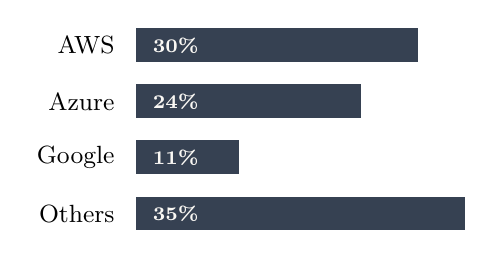
\begin{tikzpicture}[scale=0.95]
        \foreach [count=\i from 0] \v/\lab in {30/AWS,24/Azure,11/Google,35/Others} {
          \pgfmathsetmacro{\y}{2.4-0.75*\i}
          \pgfmathsetmacro{\w}{\v/35*4.4}
          \node[anchor=east,font=\small] at (-0.15,\y+0.22) {\lab};
          \draw[fill=sovDark!85,draw=none] (0,\y) rectangle (\w,\y+0.45);
          \node[anchor=west,font=\scriptsize\bfseries,text=sovPaper] at (0.1,\y+0.22) {\v\%};
        }
      \end{tikzpicture}
      \vspace{-2pt}
      {\scriptsize\color{sovGrey} Indicative global cloud infrastructure share, 2025--26 analyst estimates.}
    \end{column}
  \end{columns}
  \vspace{6pt}
  \begin{takeaway}
    \textbf{The question isn't whether we depend on cloud infrastructure --- we already do.}
    The question is \emph{whose} infrastructure, under \emph{whose} law, and who profits.
  \end{takeaway}
\end{frame}

\begin{frame}{OLK today: a working example, and its ceiling}
  \eyebrow{What we already built}
  \begin{itemize}
    \item \textbf{Open Library Kashmir} --- a privacy-first book donate/lend platform for the region. Real users, real listings, real requests.
    \item Fully open-source stack: Next.js, React, Tailwind, PostgreSQL via Supabase. Every layer is software \emph{we} control.
    \item Runs today on Supabase's hosted infrastructure --- physically in AWS's Mumbai region (\texttt{ap-south-1}).
  \end{itemize}
  \vspace{6pt}
  \eyebrow{The ceiling}
  \begin{itemize}
    \item Geographically close $\ne$ jurisdictionally ours. It is still Amazon's rack, Amazon's power, Amazon's law.
    \item Supabase itself is a US/EU company with its own terms, pricing, and continuity risk.
    \item \textbf{The good news:} because it's 100\% open-source, nothing needs to be rewritten to move it. It needs to be \emph{redeployed} --- onto infrastructure we own.
  \end{itemize}
\end{frame}

\begin{frame}{Beyond one app: why this could matter for millions}
  \begin{center}
  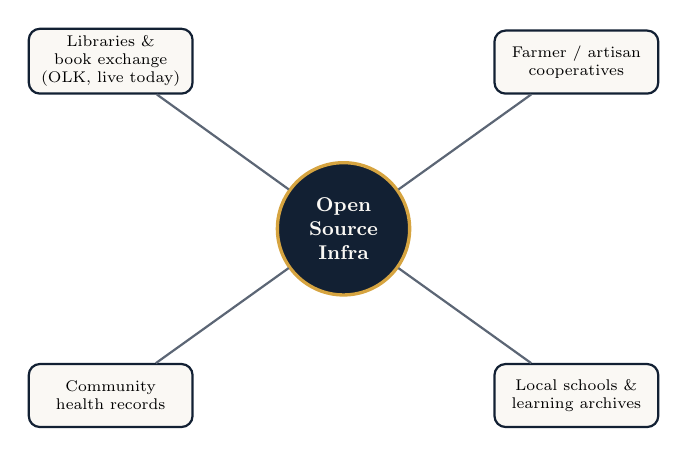
\begin{tikzpicture}[scale=0.8,every node/.style={scale=0.8}]
      \tikzset{
      hub/.style={circle,draw=sovGold,line width=1.2pt,fill=sovDark,text=sovPaper,minimum size=2.1cm,font=\small\bfseries,align=center},
      spoke/.style={rounded corners,draw=sovDark,line width=0.8pt,fill=sovPaper,minimum width=2.6cm,minimum height=1cm,font=\scriptsize,align=center},
      link/.style={draw=sovGrey,line width=0.8pt}
    }
    \node[hub] (core) {Open\\Source\\Infra};
    \node[spoke,above left=1.1cm and 1.3cm of core]  (a) {Libraries \&\\book exchange\\(OLK, live today)};
    \node[spoke,above right=1.1cm and 1.3cm of core] (b) {Farmer / artisan\\cooperatives};
    \node[spoke,below left=1.1cm and 1.3cm of core]  (c) {Community\\health records};
    \node[spoke,below right=1.1cm and 1.3cm of core] (d) {Local schools \&\\learning archives};
    \foreach \n in {a,b,c,d} \draw[link] (core) -- (\n);
  \end{tikzpicture}
  \end{center}
  \vspace{-6pt}
  \begin{takeaway}
   \footnotesize OLK is the \emph{first} baby step, not the destination. The same self-hosted stack --- Postgres, auth, storage, a web front end --- is the pattern for every community institution in the region that currently has no digital backbone of its own, from Kashmir to the wider Indian subcontinent.
  \end{takeaway}
\end{frame}

% ================================================================
\section{Internet \& Electricity: The Foundation}

\begin{frame}{How much internet do we actually need?}
  \eyebrow{Sizing the pipe for 100{,}000 users}
  \begin{columns}[T]
    \begin{column}{0.5\textwidth}
      \small
      \begin{align*}
        \text{Registered users} &= 100{,}000\\
        \text{Concurrent (peak)} &\approx 8\% = 8{,}000\\
        \text{Avg. active payload} &\approx 30~\text{KB/s/user}\\
        \text{Sustained peak} &= 8{,}000 \times 30\text{KB/s}\\
                               &\approx 240~\text{MB/s} \approx 2~\text{Gbps}\\
        \text{Burst headroom (4}\times) &\approx 8\text{--}10~\text{Gbps}
      \end{align*}
    \end{column}
    \begin{column}{0.5\textwidth}
      \begin{itemize}
        \item A typical home/business fiber line in Srinagar (100 Mbps--1 Gbps) is \textbf{an order of magnitude short} of what full scale needs.
        \item We need \textbf{datacenter-grade, redundant} uplinks: multiple carriers, multiple physical paths, not one ISP line.
        \item Kashmir's history of internet shutdowns means single-path connectivity is not just slow --- it is a single point of \emph{total} failure.
      \end{itemize}
    \end{column}
  \end{columns}
  \vspace{4pt}
  \begin{takeaway}
   \textbf{Design principle:} keep a CDN / edge cache \emph{outside} the valley (e.g.\ a Chinese cloud edge in Hong Kong or Singapore) so read-heavy traffic survives a local shutdown even if writes pause.
  \end{takeaway}
\end{frame}

\begin{frame}{Electricity: the honest picture}
  \begin{columns}[T]
    \begin{column}{0.52\textwidth}
      \eyebrow{Where J\&K's grid stands (2026)}
      \begin{itemize}
        \item Billing efficiency improved 56\% (FY21-22) $\rightarrow$ 77\% (FY25-26) under the RDSS reform program --- real progress, still not hosting-grade.
        \item KPDCL routinely issues \emph{scheduled} maintenance outages across Srinagar, Pulwama, Baramulla (e.g.\ 11--18 July 2026).
        \item Unscheduled outages remain common, especially in winter peak-load months.
      \end{itemize}
    \end{column}
    \begin{column}{0.48\textwidth}
      \eyebrow{What that means for us}
      \begin{itemize}
        \item Grid power = supplementary, not primary, from day one.
        \item Rack-level \textbf{online double-conversion UPS}, sized to full server load, minimum 30--60 min autonomy.
        \item Diesel generator, auto-transfer switch, 24--72h fuel reserve for extended outages.
        \item Solar + battery as a long-term supplement (strong insolation Apr--Oct, weak in winter --- \emph{never} the sole source).
      \end{itemize}
    \end{column}
  \end{columns}
\end{frame}

% ================================================================
\section{Physical Environment}

\begin{frame}{The room the servers live in}
  \begin{columns}[T]
    \begin{column}{0.5\textwidth}
      \eyebrow{Cooling}
      \begin{itemize}
        \item Kashmir's cool climate is an asset: free-air / economizer cooling works most of the year.
        \item Precision AC only needed for summer peak and humidity control.
        \item Sealed rack + positive-pressure filtration against valley dust and pollen.
      \end{itemize}
      \vspace{4pt}
      \eyebrow{Safety}
      \begin{itemize}
        \item Clean-agent fire suppression (FM-200/Novec) --- never water sprinklers over live racks.
        \item Smoke and heat detection wired to auto shutdown.
      \end{itemize}
    \end{column}
    \begin{column}{0.5\textwidth}
      \eyebrow{Physical security}
      \begin{itemize}
        \item Single access-controlled room; logged entry, CCTV.
        \item Locking rack cabinets; no shared building access.
        \item Humidity/temperature monitoring with SMS/email alerting.
      \end{itemize}
      \vspace{4pt}
      \begin{takeaway}
       For the \hope{pilot} (slide 29), all of this fits in a single well-prepared room with one rack --- not a purpose-built datacenter. Full 100k scale is a later, separate capital project.
      \end{takeaway}
    \end{column}
  \end{columns}
\end{frame}

% ================================================================
\section{Starting with VPS: Our On-Ramp}

\begin{frame}{Why VPS first: the staged path to sovereignty}
  \begin{center}
  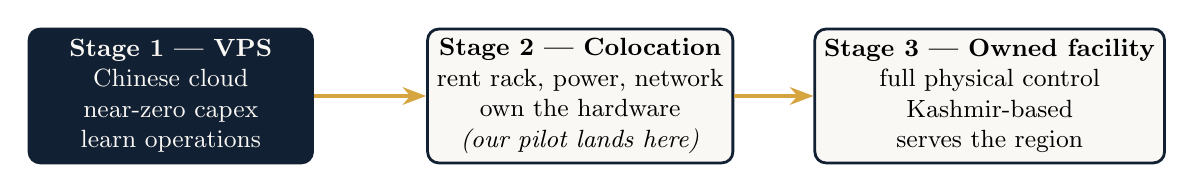
\begin{tikzpicture}[
      stage/.style={rounded corners,draw=sovDark,line width=1pt,fill=sovPaper,minimum width=3.6cm,minimum height=1.7cm,align=center,font=\small},
      hl/.style={fill=sovDark,text=sovPaper},
      arr/.style={-{Stealth[length=3mm]},line width=1.2pt,draw=sovGold}
    ]
    \node[stage,hl] (s1) at (0,0)   {\textbf{Stage 1 --- VPS}\\Chinese cloud\\near-zero capex\\learn operations};
    \node[stage]     (s2) at (5.2,0) {\textbf{Stage 2 --- Colocation}\\rent rack, power, network\\own the hardware\\\emph{(our pilot lands here)}};
    \node[stage]     (s3) at (10.4,0) {\textbf{Stage 3 --- Owned facility}\\full physical control\\Kashmir-based\\serves the region};
    \draw[arr] (s1) -- (s2);
    \draw[arr] (s2) -- (s3);
  \end{tikzpicture}
  \end{center}
  \vspace{10pt}
  \begin{itemize}
    \item \textbf{Stage 1} costs almost nothing to start and teaches the team real operational skills --- Linux, backups, monitoring --- before any capital is at risk.
    \item Every stage runs the \emph{same} open-source software stack. Moving stages is a migration, not a rewrite.
    \item We are not choosing between VPS and our own datacenter. We are choosing the \emph{order} in which we build confidence and capability.
  \end{itemize}
\end{frame}

\begin{frame}{The Chinese cloud landscape}
  \eyebrow{Why Chinese providers, specifically}
  \begin{itemize}
    \item Alibaba Cloud, Tencent Cloud and Huawei Cloud are three of the world's largest hyperscalers by capacity --- mature, globally reachable, and \textbf{outside} the US CLOUD Act's jurisdiction.
    \item All three operate international sites (Hong Kong, Singapore) purpose-built for customers outside mainland China --- no need to navigate mainland-only compliance.
    \item Huawei Cloud in particular runs on the \emph{same} CPU and OS family (Kunpeng / openEuler) we would later deploy on our own hardware --- one skill set, two stages.
    \item This is a deliberate, practical choice for this presentation: every option from here on is Chinese-made. No AWS, no Azure, no Google.
  \end{itemize}
\end{frame}

\begin{frame}{Alibaba Cloud vs.\ Tencent Cloud vs.\ Huawei Cloud}
  \small
  \renewcommand{\arraystretch}{1.25}
  \begin{tabularx}{\linewidth}{@{}l>{\raggedright\arraybackslash}X>{\raggedright\arraybackslash}X>{\raggedright\arraybackslash}X@{}}
    \toprule
     & \textbf{Alibaba Cloud} & \textbf{Tencent Cloud} & \textbf{Huawei Cloud} \\
    \midrule
    Best for us & Broadest footprint outside China; mature intl.\ billing & \texttt{Lighthouse} = simple all-in-one VPS, ideal first pilot & Kunpeng + openEuler = same stack as our own future hardware \\
    Nearby region & Singapore, Hong Kong & Hong Kong, Singapore & Hong Kong, Singapore \\
    Est.\ latency to Srinagar & $\sim$40--80\,ms & $\sim$40--80\,ms & $\sim$40--80\,ms \\
    Entry product & ECS (Elastic Compute Service) & CVM / Lighthouse & ECS (incl.\ Kunpeng instances) \\
    Support in English & Good & Good & Improving \\
    \bottomrule
  \end{tabularx}
  \vspace{10pt}
  \begin{takeaway}
   \textbf{Recommendation:} start on \emph{Tencent Lighthouse} or \emph{Alibaba ECS} for the cheapest, fastest first pilot; plan the eventual on-prem hardware around \emph{Huawei's} Kunpeng/openEuler ecosystem for continuity.
  \end{takeaway}
\end{frame}

\begin{frame}{Getting a Chinese VPS as a foreign, non-mainland user}
  \eyebrow{Practical steps}
  \begin{enumerate}
    \item Register on the \textbf{international} site (\texttt{intl.alibabacloud.com}, \texttt{intl.cloud.tencent.com}, \texttt{huaweicloud.com/intl}) --- not the mainland site.
    \item Choose a \textbf{Hong Kong or Singapore} region: this avoids China's mainland \textbf{ICP license} requirement, which only applies to sites physically hosted inside mainland China.
    \item Identity verification: passport + organisation documents (we would register OLK/the collective formally to do this cleanly).
    \item Payment: international credit card; PayPal or Alipay-linked options exist on some products.
    \item Start \textbf{pay-as-you-go} on a small instance before committing to any reserved/annual plan --- validate our workload first.
  \end{enumerate}
  \vspace{6pt}
  \begin{takeaway}
    None of this requires a China-based business entity. It requires an afternoon of paperwork.
  \end{takeaway}
\end{frame}

% ================================================================
\section{Hardware for Full Scale: 100{,}000 Users}

\begin{frame}{Storage 101: what we need, and how much}
  \begin{columns}[T]
    \begin{column}{0.48\textwidth}
      \eyebrow{SSD vs.\ NVMe}
      \begin{itemize}
        \item SATA SSD: fast, cheap, capped around 550\,MB/s by the SATA interface.
        \item \textbf{NVMe}: talks directly over PCIe lanes --- multi-\si{\giga\byte\per\second} throughput and far higher IOPS. Essential for a database doing thousands of small random reads/writes (exactly our workload).
      \end{itemize}
    \end{column}
    \begin{column}{0.52\textwidth}
      \eyebrow{Sizing for 100{,}000 users}
      \small
      \begin{itemize}
        \item Avg.\ user footprint (profile + listings + messages) $\approx$ 5\,MB $\rightarrow$ 500\,GB
        \item Book cover images, $\sim$300k listings $\times$ 300\,KB $\approx$ 90\,GB
        \item DB overhead: indexes, WAL, replication, backups ($3$--$5\times$)
        \item \textbf{Design target: 2--5\,TB hot NVMe}, plus a separate warm/archive tier for older data and backups
      \end{itemize}
    \end{column}
  \end{columns}
  \begin{takeaway}
   This is exactly why our pilot's \textbf{5\,TB NVMe} spec (slide 29) isn't arbitrary --- it is sized with real headroom for 10--20k users today and a clear growth path toward 100k.
  \end{takeaway}
\end{frame}

\begin{frame}{RAID: redundancy is not optional}
  \small
  \renewcommand{\arraystretch}{1.2}
  \begin{tabularx}{\linewidth}{@{}l>{\raggedright\arraybackslash}X cc@{}}
    \toprule
    \textbf{Level} & \textbf{How it works} & \textbf{Fault tolerance} & \textbf{Usable capacity} \\
    \midrule
    RAID 0 & Striped, no redundancy & None & 100\% \\
    RAID 1 & Mirrored pair & 1 disk & 50\% \\
    RAID 5 & Striped + 1 parity disk & 1 disk & $(n-1)/n$ \\
    RAID 6 & Striped + 2 parity disks & 2 disks & $(n-2)/n$ \\
    \textbf{RAID 10} & Mirrored pairs, then striped & 1 per mirror & 50\% \\
    \bottomrule
  \end{tabularx}
  \vspace{10pt}
  \begin{takeaway}
   \textbf{Our pick:} RAID 10 for the live database volume --- best performance \emph{and} redundancy, worth the capacity cost for the system of record. RAID 6 is acceptable for the bulk image/backup archive, where raw capacity matters more than latency.
  \end{takeaway}
\end{frame}

\begin{frame}{ECC RAM: why a bit-flip matters here}
  \begin{itemize}
    \item Consumer RAM has no protection against random bit-flips caused by cosmic rays or electrical noise --- rare, but real, and worse at scale (more DIMMs, more hours of uptime).
    \item \textbf{ECC (Error-Correcting Code) RAM} detects and silently corrects single-bit errors in real time.
    \item For a \emph{system of record} --- who owns which book, who borrowed what --- a silently corrupted row is far worse than a slow page load. This is not a place to save money.
  \end{itemize}
  \vspace{8pt}
  \eyebrow{Sizing}
  \begin{itemize}
    \item PostgreSQL wants RAM close to its working set. \textbf{128\,GB} gives $\sim$32\,GB \texttt{shared\_buffers} plus generous OS page cache --- comfortable for the 10--20k pilot.
    \item Full 100k scale: 256--512\,GB per node, or split the workload across several nodes with a distributed database (slide 24) instead of one ever-bigger box.
  \end{itemize}
\end{frame}

\begin{frame}{The Chinese hardware stack, end to end}
  \small
  \renewcommand{\arraystretch}{1.3}
  \begin{tabularx}{\linewidth}{@{}l>{\raggedright\arraybackslash}X@{}}
    \toprule
    \textbf{Layer} & \textbf{Chinese-made option} \\
    \midrule
    CPU & Huawei \textbf{Kunpeng} 920/950 (ARM64; the new TaiShan 950 SuperPoD ships up to 192-core/384-thread, Q1 2026) \\
    Server chassis & Huawei \textbf{TaiShan}, \textbf{Inspur}, \textbf{XFusion} (H3C) --- all ship Kunpeng/openEuler-certified rack servers \\
    Storage & \textbf{YMTC / ZhiTai} NVMe --- domestic 3D NAND (Xtacking 4.0); flagship PCIe 5.0 models reach $\sim$10--15\,GB/s reads \\
    Operating system & \textbf{openEuler} --- Huawei's open-source Linux, ARM64-native, $>$50\% share of newly deployed China server OS (IDC, 2024) \\
    Networking & Huawei / H3C switches, 10--25\,GbE \\
    \bottomrule
  \end{tabularx}
  \begin{takeaway}
    Kunpeng-based servers already hold over 20\% of the China server market (IDC, 2024) --- this is not a fringe or unproven stack, it is mainstream infrastructure we can simply choose.
  \end{takeaway}
\end{frame}

\begin{frame}{A concrete Bill of Materials --- 100k-scale node}
  \small
  \renewcommand{\arraystretch}{1.3}
  \begin{tabularx}{\linewidth}{@{}l>{\raggedright\arraybackslash}X@{}}
    \toprule
    \textbf{Component} & \textbf{Spec} \\
    \midrule
    Chassis & 2U TaiShan / XFusion rack server, dual PSU \\
    CPU & 1--2$\times$ Kunpeng 920-class (ARM64) \\
    RAM & 256\,GB ECC RDIMM \\
    Boot volume & 2$\times$ enterprise SATA SSD, RAID 1 \\
    Database volume & 6$\times$ ZhiTai/YMTC NVMe, RAID 10 ($\sim$5--8\,TB usable) \\
    Network & Dual-port 10/25\,GbE \\
    OS & openEuler LTS \\
    Rack support & UPS (online double-conversion) + PDU \\
    \bottomrule
  \end{tabularx}
  \vspace{12pt}
  {\scriptsize\color{sovGrey} Pricing fluctuates with CNY/INR rates and is best obtained as a direct quote from an XFusion/Inspur reseller or a Huawei Cloud dedicated-host equivalent --- treat this as a specification, not a quote.}
\end{frame}

% ================================================================
\section{Software \& the Skills We Need}

\begin{frame}{The software stack: what changes, what doesn't}
  \begin{columns}[T]
    \begin{column}{0.5\textwidth}
      \eyebrow{Stays the same}
      \begin{itemize}
        \item \textbf{PostgreSQL} --- what Supabase runs today, and what OLK already depends on. Open-source, portable, battle-tested.
        \item Our entire app layer (Next.js, Auth, Storage APIs) is already license-free to redeploy anywhere.
      \end{itemize}
    \end{column}
    \begin{column}{0.5\textwidth}
      \eyebrow{New, Chinese, and worth knowing}
      \begin{itemize}
        \item \textbf{openGauss} --- Huawei's own PostgreSQL fork, built for distributed, PB-scale workloads.
        \item \textbf{TiDB} (PingCAP) --- MySQL-wire-compatible distributed SQL, strong open-source community.
        \item \textbf{OceanBase} (Ant Group) --- financial-grade distributed OLTP at extreme concurrency.
      \end{itemize}
    \end{column}
  \end{columns}
  \vspace{8pt}
  \begin{takeaway}
   \textbf{Because openGauss is a PostgreSQL fork, our migration path exists but isn't urgent.} We only need to reach for a distributed database like this once a single well-specced node (our pilot) stops being enough --- likely well past 100k users.
  \end{takeaway}
\end{frame}

\begin{frame}{Supabase self-hosting: we are already sovereignty-ready}
  \begin{itemize}
    \item Supabase is a thin, open-source layer over Postgres: \texttt{PostgREST} (API), \texttt{GoTrue} (auth), \texttt{Realtime}, \texttt{Storage API}, \texttt{Studio} --- all Apache/MIT licensed, all Docker-composable.
    \item We already run this \emph{exact} stack locally via the Supabase CLI and Docker for development.
    \item Self-hosting in production is the same containers, pointed at our own Postgres, on our own machine, behind our own domain.
  \end{itemize}
  \vspace{10pt}
  \begin{takeaway}
   \textbf{The headline point of this whole talk:} we do not need to rewrite Open Library Kashmir to make it sovereign. We need to \emph{redeploy} it --- onto a VPS first, then our own hardware.
  \end{takeaway}
\end{frame}

\begin{frame}{Skills matrix: what our team must build}
  \small
  \renewcommand{\arraystretch}{1.25}
  \begin{tabularx}{\linewidth}{@{}>{\raggedright\arraybackslash}X>{\raggedright\arraybackslash}X c@{}}
    \toprule
    \textbf{Skill} & \textbf{Why it's needed} & \textbf{Have today?} \\
    \midrule
    Linux / openEuler administration & Every layer runs on it & Partial \\
    Docker \& container orchestration & How Supabase's services are deployed & Yes \\
    PostgreSQL DBA (backup, tuning, replication) & Data integrity at scale & Partial \\
    Networking \& firewalling (multi-carrier failover) & Shutdown-resilient uplink & No --- to learn \\
    Security (patching, encryption at rest, intrusion detection) & System of record for real people & No --- to learn \\
    Facilities basics (power, cooling) & Slides 9 \& 11 & No --- to learn \\
    \bottomrule
  \end{tabularx}
  \vspace{8pt}
  \begin{takeaway}
   This is a call for volunteers as much as it is a call for hardware budget. Every gap in the ``No'' column is a role someone in this room could own.
  \end{takeaway}
\end{frame}

\begin{frame}{Backups \& disaster recovery}
  \eyebrow{The 3-2-1 rule, adapted for us}
  \begin{itemize}
    \item \textbf{3} copies of the data --- production + two backups.
    \item \textbf{2} different media/locations --- e.g.\ local NVMe snapshot + a separate disk or machine.
    \item \textbf{1} copy offsite --- a different city in J\&K, or an \textbf{encrypted} bucket on Alibaba OSS / Tencent COS, used strictly as cold backup storage, never as the primary host.
  \end{itemize}
  \vspace{10pt}
  \begin{takeaway}
   Everything is encrypted \emph{before} it leaves our building. An offsite Chinese cloud bucket used purely for encrypted backup carries none of the sovereignty compromise of hosting live traffic there.
  \end{takeaway}
\end{frame}

% ================================================================
\section{The Hope}

\begin{frame}{The proposal: one machine, real capacity, right now}
  \begin{columns}[T]
    \begin{column}{0.53\textwidth}
      \eyebrow{The pilot}
      \begin{itemize}
        \item \textbf{10{,}000--20{,}000 users}, served from a \emph{single} well-specced machine.
        \item \textbf{5\,TB usable NVMe} (RAID 10) + \textbf{128\,GB ECC RAM} + Kunpeng-class CPU, openEuler, PostgreSQL + self-hosted Supabase.
        \item Chinese-made hardware and hosting throughout --- no Western dependency, from the VM to the silicon.
      \end{itemize}
    \end{column}
    \begin{column}{0.47\textwidth}
      \eyebrow{Why this scope}
      \begin{itemize}
        \item Small enough to fund and operate with volunteer skills we can build this year.
        \item Large enough to be a \emph{real} platform, not a toy demo.
        \item Proves every claim in this talk before we ask for datacenter-scale capital.
      \end{itemize}
    \end{column}
  \end{columns}
  \vspace{6pt}
  \small
  \renewcommand{\arraystretch}{1.15}
  \begin{tabularx}{\linewidth}{@{}l>{\raggedright\arraybackslash}X@{}}
    \toprule
    Headroom & $20{,}000~\text{users} \times 5~\text{MB} \approx 100$\,GB active data $\rightarrow$ $5$\,TB $/$ $100$\,GB $\approx \mathbf{50\times}$ headroom \\
    \bottomrule
  \end{tabularx}
  {\scriptsize\color{sovGrey} Enough for years of growth, every book cover, every backup snapshot, without touching the hardware again.}
\end{frame}

\begin{frame}{The road from here}
  \begin{center}
  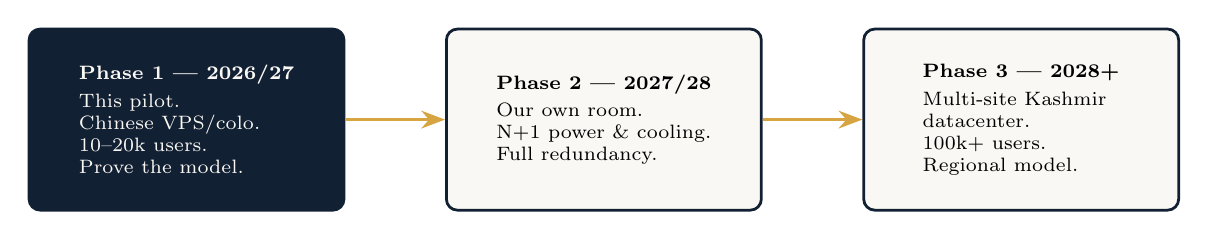
\begin{tikzpicture}[
      ph/.style={rounded corners,draw=sovDark,line width=1pt,fill=sovPaper,minimum width=4cm,minimum height=2.3cm,align=left,font=\scriptsize,inner sep=6pt},
      hl/.style={fill=sovDark,text=sovPaper},
      arr/.style={-{Stealth[length=3mm]},line width=1.2pt,draw=sovGold}
    ]
    \node[ph,hl] (p1) at (0,0)   {\textbf{Phase 1 --- 2026/27}\\[2pt] This pilot.\\ Chinese VPS/colo.\\ 10--20k users.\\ Prove the model.};
    \node[ph]     (p2) at (5.3,0) {\textbf{Phase 2 --- 2027/28}\\[2pt] Our own room.\\ N+1 power \& cooling.\\ Full redundancy.};
    \node[ph]     (p3) at (10.6,0) {\textbf{Phase 3 --- 2028+}\\[2pt] Multi-site Kashmir\\ datacenter.\\ 100k+ users.\\ Regional model.};
    \draw[arr] (p1) -- (p2);
    \draw[arr] (p2) -- (p3);
  \end{tikzpicture}
  \end{center}
  \vspace{10pt}
  \begin{takeaway}
   \hope{What we're asking for tonight:} a funding commitment for the Phase 1 bill of materials, volunteers against the skills matrix, and a room to eventually call our own. This is buildable in months, not decades --- and it starts the moment we agree to start.
  \end{takeaway}
  \vspace{6pt}
  \centering
  {\large Our data. Our servers. Our region. \color{sovGold}\textbf{Let's begin.}}
\end{frame}

\end{document}
